\section{Introduction}
\label{sec:introduction_010}

Discrete events, occurring irregularly over time, are a common data type generated naturally in our everyday interactions with the environment (see Fig.~\ref{fig:model_illustration_1} for an illustration). Examples include messages in social networks, medical histories of patients in healthcare, and integrated information from multiple sensors in complex systems like cars. The problem we are solving in this work is: given a (past) sequence of asynchronous events, what will happen next? Answering this question enables us to predict, e.g., what action an internet user will likely perform or which part of a car might fail.

While many recurrent models for asynchronous sequences have been proposed in the past \cite{PhasedLstm, RMTPP}, they are ill-suited for this task since they output a \textit{single prediction} (e.g.\ the most likely next event) only. In an asynchronous setting, however, such a single prediction is not enough since the most likely event can change with the passage of time -- even if no other events happen. Consider a car approaching another vehicle in front of it. Assuming nothing happens in the meantime, we can expect different events at \textit{different times in the future}. When forecasting a short time, one expects the driver to start overtaking; after a longer time one would expect braking; in the long term, one would expect a collision. Thus, the expected behavior changes depending on the time we forecast, assuming no events occured in the meantime. Fig.\ \ref{fig:model_illustration_1} illustrates this schematically: having observed a square and a pentagon, it is likely to observe a square after a short time, while a circle after a longer time. Clearly, if some event occurs, e.g.\ braking/square, the event at the (then) observed time will be taken into account, updating the temporal prediction.

An ad-hoc solution to this problem would be to discretize time. However, if the events are near each other, a high sampling frequency is required, giving us very high computational cost. Besides, since there can be intervals without events, an artificial `no event' class is required.

In this work, we solve these problems by directly predicting the entire evolution of the events over (continuous) time. Given a past asynchronous sequence as input, we can predict and evaluate for \textit{any} future timepoint what the next event will likely be (under the assumption that no other event happens in between which would lead to an update of our model). Crucially, the likelihood of the events might change and one event can be more likely than others multiple times in the future. This periodicity exists in many event sequences. For instance, given that a person is currently at home, a smart home would predict a high probability that the kitchen will be used at lunch and/or dinner time (see Fig.\ \ref{fig:kitchen_categorical} for an illustration). We require that our model captures such multimodality.

\begin{wrapfigure}[13]{r}{7cm}
        \vspace{-0.5cm}
        \centering
        % \begin{subfigure}{.25 \linewidth}
        %       \centering
        %     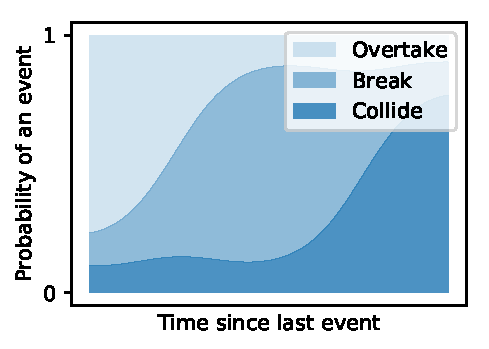
\includegraphics[width=\linewidth]{images/categorical_evolution.pdf}
        %     \vspace*{-0.6cm}
        %     \caption{}
        %     \label{fig:car_categorical}
        % \end{subfigure}
        \begin{subfigure}{.5 \linewidth}
                \centering
                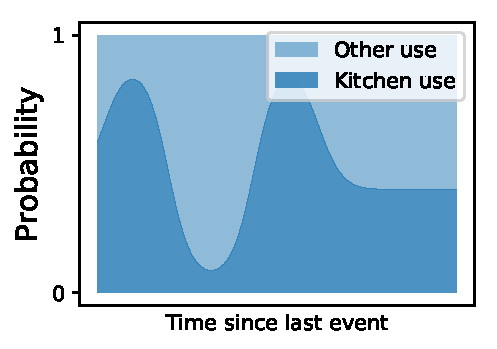
\includegraphics[width=\linewidth]{sections/010_neurips2019/paper/images/categorical_evolution2.pdf}
                \vspace*{-0.6cm}
                \caption{}
                \label{fig:kitchen_categorical}
        \end{subfigure}
        % \hspace{0.3cm}
        \begin{subfigure}{.4 \linewidth}
                \centering
                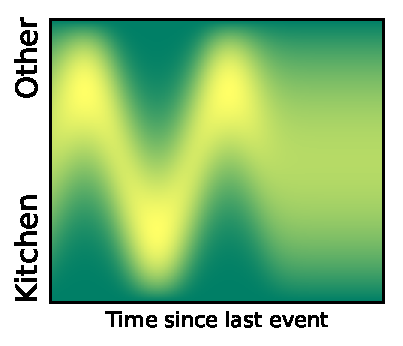
\includegraphics[width=\linewidth]{sections/010_neurips2019/paper/images/dirichlet_evolution.pdf}
                \vspace*{-0.6cm}
                \caption{}
                \label{fig:kitchen_uncertainty}
        \end{subfigure}
        %\vspace{-0.2cm}
        \caption{(a) An event can be expected multiple times in the future. (b) At some times we should be uncertain in the prediction. Yellow denotes higher probability density.}
        % \vspace*{-0.6cm}
\end{wrapfigure}
While Fig.\ \ref{fig:kitchen_categorical} illustrates the evolution of the categorical distribution (corresponding to the probability of a specific event class to happen), an issue still arises outside of the observed data distribution. {E.g.\ in some time intervals we can be \textit{certain} that two classes are \textit{equiprobable}, having observed many similar examples. However,} if the model has not seen any examples at specific time intervals during training, we do not want to give a confident prediction. Thus, we incorporate \textit{uncertainty} in a prediction directly in our model. In places where we expect events, the confidence will be higher, and outside of these areas the uncertainty in a prediction will grow as illustrated in Fig.\ \ref{fig:kitchen_uncertainty}. Technically, instead of modeling the evolution of a categorical distribution, we model the \textit{evolution of a distribution on the probability simplex}.
%
Overall, our model enables us to operate with the \textit{asynchronous discrete} event data from the past as input to perform \textit{continuous-time} predictions to the future incorporating the predictions' uncertainty. This is in contrast to existing works as \cite{RMTPP, hawkes}.
